This section provides context to the origin of the idea of a unified algorithmic framework for complex systems.

%%%%%%% Put what I wrote here
\begin{figure}[thpb]
  \centering
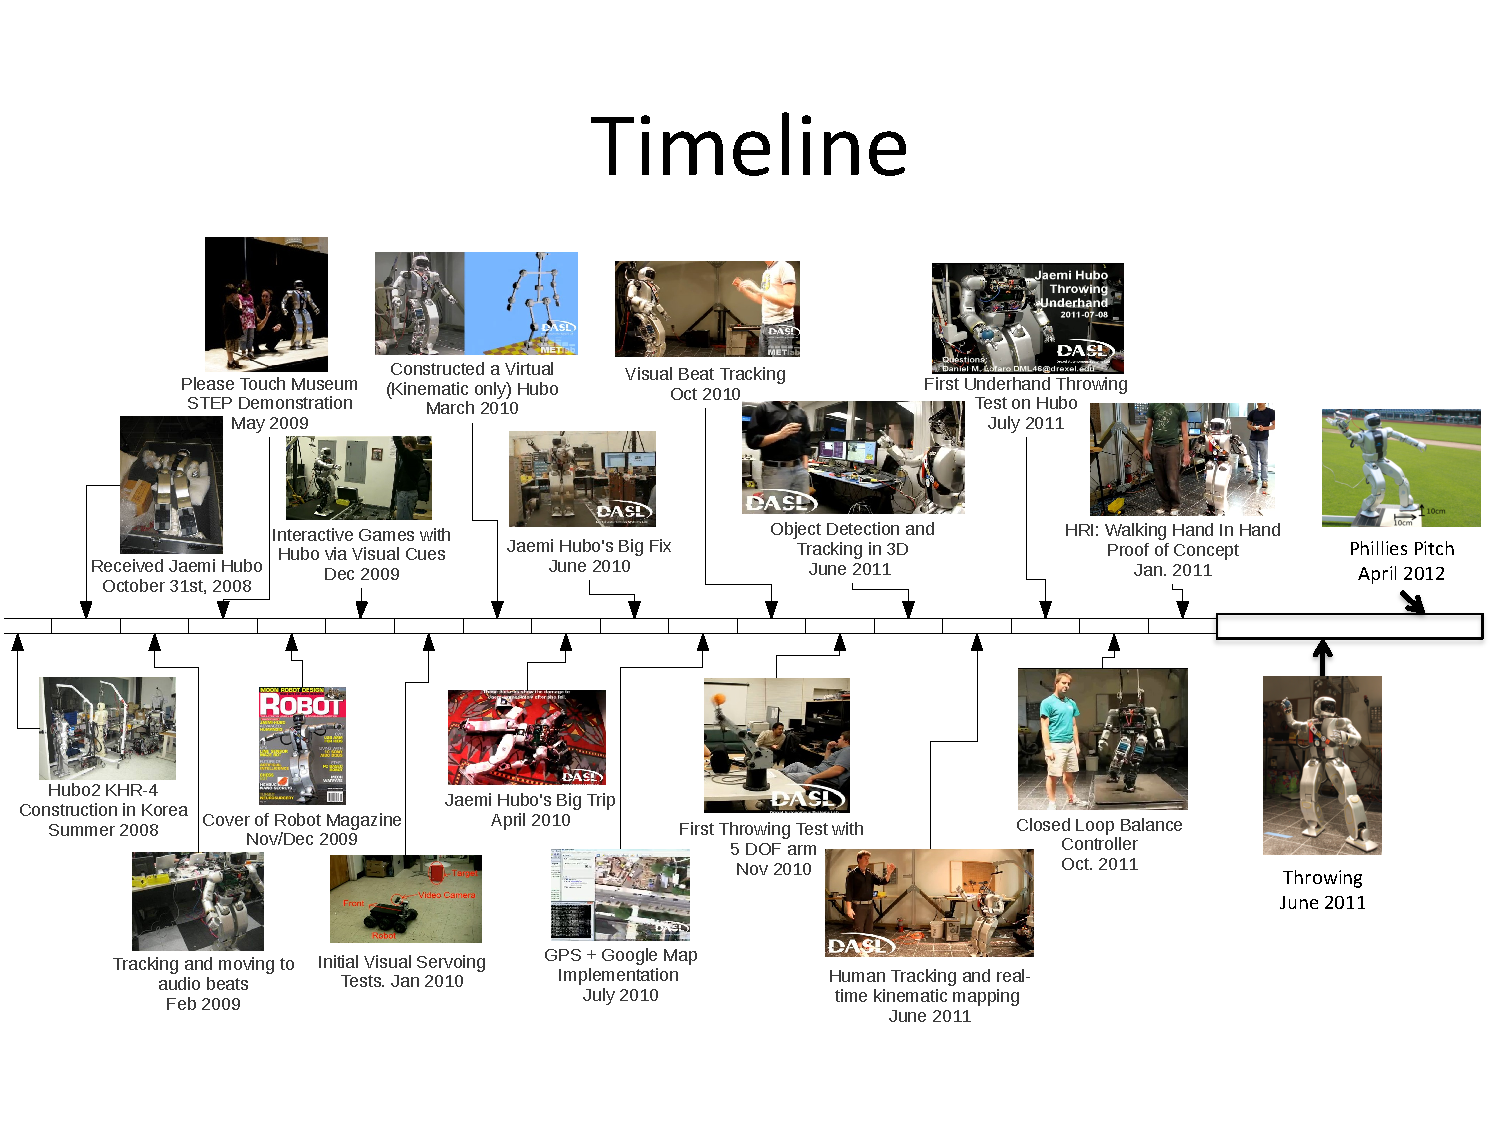
\includegraphics[angle=90, width=0.9\columnwidth]{./pix/Timeline.pdf}
  \caption{Timeline of Daniel M. Lofaro's research from 2008 to 2012}
  \label{fig:timeline}
\end{figure}

\subsection{Human Robot Interaction}
The initial goal was to have a humanoid robot become an interactive musical participant with humans.
This spawned the creation of a visual method of tracking the beat in the absence of auditory cues\cite{5686847}.
This came from a modification of a method of allowing children to play interactive games with humanoid robots\cite{lofaroGamesRobot}.
The resulting method was effective, but to increase the accuracy it was required to combine a pre-existing auditory beat tracker with the visual system.
This calumniated with a multi process system that combine the auditory and visual beat trackers\cite{lofaroIASTED2011,6094987,lofaroEURASIP2011}.
A human comparison was completed and found that this combined method was as accurate at detecting the beat in music as average humans.

\subsubsection{Results from preliminary experiments}
When collaborating with other to create a complex robot control systems integrating controllers is difficult because of the use of:
\begin{itemize}
\item different loop rates causing synchronization issues
\item different programming languages making using the same libraries a challenge
\end{itemize}

It was found that it is best to keep each working systems \textit{independent} allowing them to run at their native rate and on their native platforms\cite{ach}.



\subsection{High Degree of Freedom Kinematic Planning}
The next challenge was to perform kinematic planning for end effector velocity control. 
This resulted in the development of a method that is able to solve inverse kinematics (IK) for high degree of freedom (DOF) systems where there is no closed-form solution as well as create collision free trajectories for high DOF robots\cite{6385987}.
This is described in detail in Section~\ref{sec:srm} and \ref{sec:baseball}.
This culminated in the verification and validation of the system by an experiment where Hubo full-size humanoid robot throw the first pitch at a Major League Baseball (MLB) game\cite{lofaroHumanoids2012,6462956}.

\subsubsection{Results from preliminary experiments}
As best practice when controllers and planners are implemented it is important that low-level controllers such as balance and obstacle avoidance run at all times\cite{lofaroRAM2013}. 
Non-priority controllers such as throwing trajectory planning can run in the background in a separate process.
Keeping the processes separate allowed the system to be more resistant to lag and crashes of one or more of the controllers.
This brought validation to the overarching plan for the unified algorithmic framework for complex systems and humanoid robots.




\subsection{Lessons Learned}

At this point creating these experiment it was required to \textit{hacked} together pre-existing systems that allowed the robot to do the task.
This is the point where it was realized that a \textit{unified algorithmic framework for complex systems and humanoid robots} was required for further development in the field.
Key lessons learned from these experiments were:
\begin{itemize}
\item Must inherently decouple controllers loop rates and phases
\item Must allow for collaborators not have to \textit{inject} their code into existing source.
\item Must work with multiple robots for testing, evaluation, validation, and verification.
\end{itemize}

\noindent This is where Hubo-Ach was born.
The idea was to create a multi process architecture for humanoid control using state of the art high-speed low-latency Inter-Process Communication (IPC) techniques\cite{lofaroRAM2013}.
This is different from traditional IPC techniques because of the lack of head of line (HOL) blocking and focus on low-latency.
Section~\ref{sec:ipc} gives further details and comparisons of different IPCs.


The need for this unified framework was amplified when the Hubo was chosen to be the primary platform for the DRC-Hubo\footnote{DRC-Hubo: http://www.drc-hubo.com/} Track-A team.
Since its initial conception Hubo-Ach has become a fully functional system used in active research by multiple universities including MIT, WPI, Purdue, Ohio State, Swarthmore College, Georgia Tech, and Drexel University\cite{lofaroTePRA2013HuboAch,lofaroTePRA2013Valve}.
This research also acts as a key source of verification and validation of the system.

